% Extension decision tree — compact cheat-sheet variant.
% Same 5 questions, shorter wording, abbreviated extension paths.
\documentclass[tikz,border=4mm]{standalone}
\usepackage{tikz}
\usetikzlibrary{positioning, shapes.geometric, arrows.meta, calc}

\begin{document}
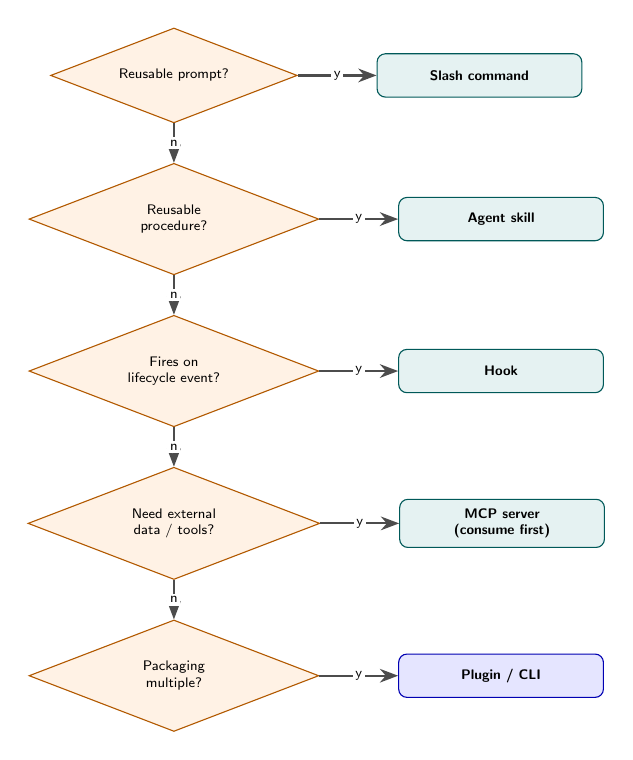
\begin{tikzpicture}[
  font=\sffamily,
  node distance=0.5cm and 1.0cm,
  question/.style={
    draw=orange!70!black, fill=orange!10, diamond, aspect=2.6,
    inner sep=0.5pt, align=center, text width=2.6cm, font=\sffamily\tiny
  },
  pattern/.style={
    draw=teal!70!black, fill=teal!10, rounded corners=3pt,
    minimum width=2.6cm, minimum height=0.55cm, align=center,
    font=\sffamily\tiny\bfseries
  },
  packaging/.style={pattern,
    draw=blue!70!black, fill=blue!10
  },
  arrow/.style={-Stealth, thick, draw=gray!60!black},
  arrowlabel/.style={font=\sffamily\tiny, fill=white, inner sep=1pt},
]

\node[question] (q1) {Reusable prompt?};
\node[pattern, right=of q1] (cmd) {Slash command};

\node[question, below=of q1] (q2) {Reusable \\ procedure?};
\node[pattern, right=of q2] (skill) {Agent skill};

\node[question, below=of q2] (q3) {Fires on \\ lifecycle event?};
\node[pattern, right=of q3] (hook) {Hook};

\node[question, below=of q3] (q4) {Need external \\ data / tools?};
\node[pattern, right=of q4] (mcp) {MCP server \\ \tiny(consume first)};

\node[question, below=of q4] (q5) {Packaging \\ multiple?};
\node[packaging, right=of q5] (plug) {Plugin / CLI};

\draw[arrow] (q1) -- node[arrowlabel] {y} (cmd);
\draw[arrow] (q1) -- node[arrowlabel] {n} (q2);
\draw[arrow] (q2) -- node[arrowlabel] {y} (skill);
\draw[arrow] (q2) -- node[arrowlabel] {n} (q3);
\draw[arrow] (q3) -- node[arrowlabel] {y} (hook);
\draw[arrow] (q3) -- node[arrowlabel] {n} (q4);
\draw[arrow] (q4) -- node[arrowlabel] {y} (mcp);
\draw[arrow] (q4) -- node[arrowlabel] {n} (q5);
\draw[arrow] (q5) -- node[arrowlabel] {y} (plug);

\end{tikzpicture}
\end{document}
